\documentclass[border=10pt]{standalone}
\usepackage[svgnames]{xcolor}
\usepackage{amsmath}
\usepackage{pgfplots}
\pgfplotsset{compat=newest}
\usepackage[sfdefault]{FiraSans}
\usepackage{FiraMono}
\renewcommand*\familydefault{\sfdefault}
\begin{document}
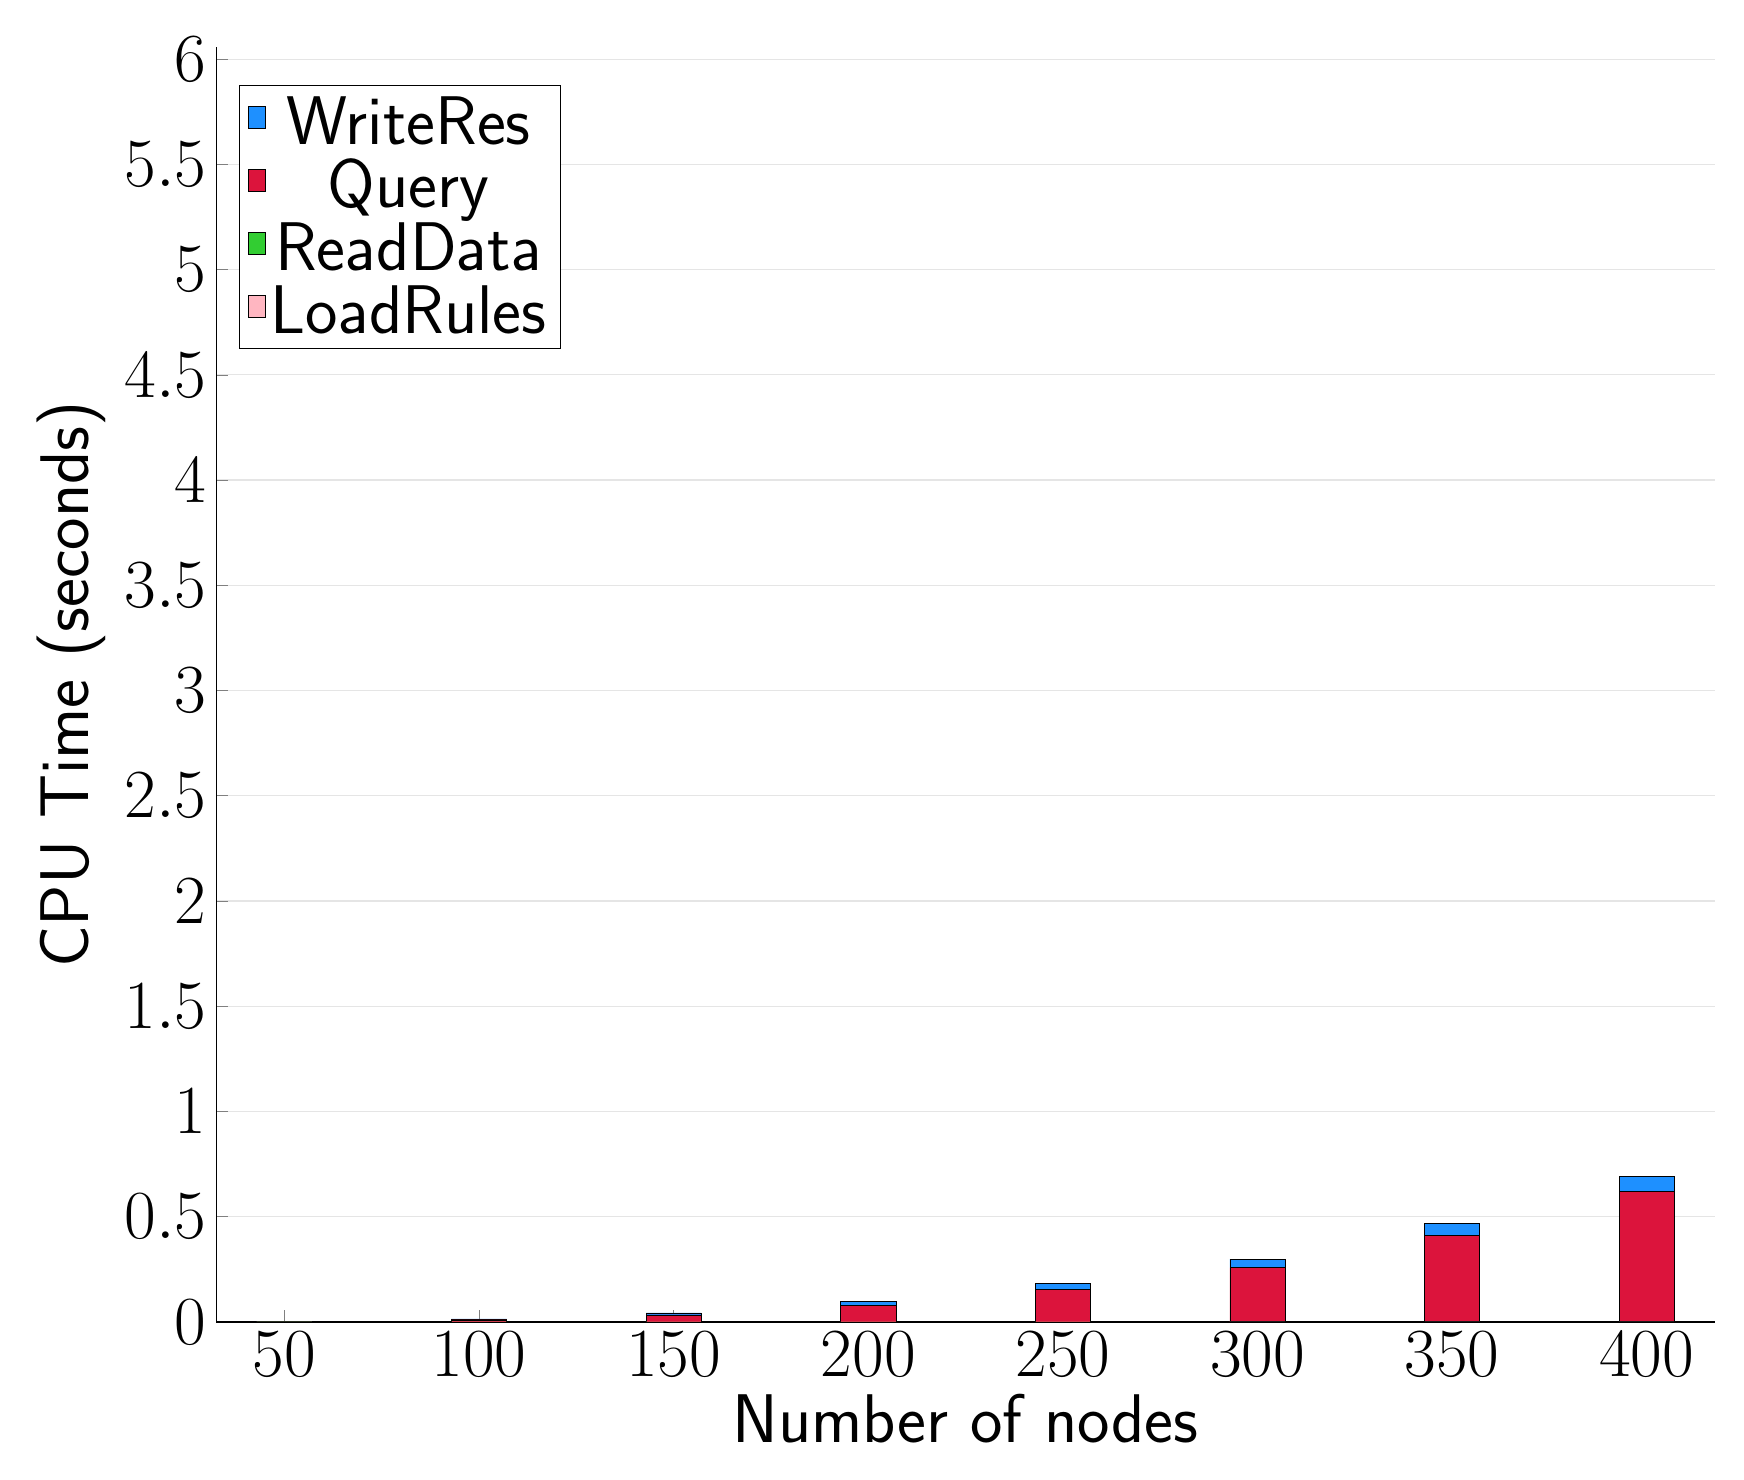
\begin{tikzpicture}
\begin{axis}[
   ybar stacked,
   width=1.7\textwidth,
   bar width=0.7cm,
   ymajorgrids, tick align=inside,
   major grid style={draw=gray!20},
   xtick=data,
   ymin=0, ymax=6.059334,
   axis x line*=bottom,
   axis y line*=left,
   enlarge x limits=0.05,
   legend style={
       at={(0.23, 0.97)},
       anchor=north east,
       legend columns=1,
       font=\Huge,
   },
   ylabel={CPU Time (seconds)},
   xlabel={Number of nodes},
   label style={font=\Huge},
   tick label style={font=\Huge},
]
\addlegendimage{fill=DodgerBlue, draw=black, line width=0.2pt}
\addlegendentry{WriteRes}
\addlegendimage{fill=Crimson, draw=black, line width=0.2pt}
\addlegendentry{Query}
\addlegendimage{fill=LimeGreen, draw=black, line width=0.2pt}
\addlegendentry{ReadData}
\addlegendimage{fill=LightPink, draw=black, line width=0.2pt}
\addlegendentry{LoadRules}
\addplot +[fill=LightPink, draw=black, line width=0.2pt] coordinates {
(50, 0.0005971999999999998)
(100, 0.0006169999999999998)
(150, 0.0005948000000000001)
(200, 0.0006047000000000003)
(250, 0.0006054000000000003)
(300, 0.0006120000000000003)
(350, 0.0006151000000000002)
(400, 0.0006180000000000001)
};
\addplot +[fill=LimeGreen, draw=black, line width=0.2pt] coordinates {
(50, 0.0001718)
(100, 0.0002208)
(150, 0.0002559000000000001)
(200, 0.00030809999999999985)
(250, 0.00034659999999999997)
(300, 0.00039219999999999994)
(350, 0.00043989999999999947)
(400, 0.0004864999999999994)
};
\addplot +[fill=Crimson, draw=black, line width=0.2pt] coordinates {
(50, 0.0012109999999999998)
(100, 0.0095396)
(150, 0.03263)
(200, 0.07761490000000001)
(250, 0.15253049999999999)
(300, 0.25664099999999995)
(350, 0.4110653)
(400, 0.6193593000000001)
};
\addplot +[fill=DodgerBlue, draw=black, line width=0.2pt] coordinates {
(50, 0.0011376)
(100, 0.004636500000000002)
(150, 0.009911)
(200, 0.018389199999999998)
(250, 0.028097499999999997)
(300, 0.04093370000000001)
(350, 0.055071400000000006)
(400, 0.0723582)
};
\end{axis}
\end{tikzpicture}

\end{document}
